\documentclass[twoside]{book}

% Packages required by doxygen
\usepackage{fixltx2e}
\usepackage{calc}
\usepackage{doxygen}
\usepackage[export]{adjustbox} % also loads graphicx
\usepackage{graphicx}
\usepackage[utf8]{inputenc}
\usepackage{makeidx}
\usepackage{multicol}
\usepackage{multirow}
\PassOptionsToPackage{warn}{textcomp}
\usepackage{textcomp}
\usepackage[nointegrals]{wasysym}
\usepackage[table]{xcolor}

% Font selection
\usepackage[T1]{fontenc}
\usepackage[scaled=.90]{helvet}
\usepackage{courier}
\usepackage{amssymb}
\usepackage{sectsty}
\renewcommand{\familydefault}{\sfdefault}
\allsectionsfont{%
  \fontseries{bc}\selectfont%
  \color{darkgray}%
}
\renewcommand{\DoxyLabelFont}{%
  \fontseries{bc}\selectfont%
  \color{darkgray}%
}
\newcommand{\+}{\discretionary{\mbox{\scriptsize$\hookleftarrow$}}{}{}}

% Page & text layout
\usepackage{geometry}
\geometry{%
  a4paper,%
  top=2.5cm,%
  bottom=2.5cm,%
  left=2.5cm,%
  right=2.5cm%
}
\tolerance=750
\hfuzz=15pt
\hbadness=750
\setlength{\emergencystretch}{15pt}
\setlength{\parindent}{0cm}
\setlength{\parskip}{3ex plus 2ex minus 2ex}
\makeatletter
\renewcommand{\paragraph}{%
  \@startsection{paragraph}{4}{0ex}{-1.0ex}{1.0ex}{%
    \normalfont\normalsize\bfseries\SS@parafont%
  }%
}
\renewcommand{\subparagraph}{%
  \@startsection{subparagraph}{5}{0ex}{-1.0ex}{1.0ex}{%
    \normalfont\normalsize\bfseries\SS@subparafont%
  }%
}
\makeatother

% Headers & footers
\usepackage{fancyhdr}
\pagestyle{fancyplain}
\fancyhead[LE]{\fancyplain{}{\bfseries\thepage}}
\fancyhead[CE]{\fancyplain{}{}}
\fancyhead[RE]{\fancyplain{}{\bfseries\leftmark}}
\fancyhead[LO]{\fancyplain{}{\bfseries\rightmark}}
\fancyhead[CO]{\fancyplain{}{}}
\fancyhead[RO]{\fancyplain{}{\bfseries\thepage}}
\fancyfoot[LE]{\fancyplain{}{}}
\fancyfoot[CE]{\fancyplain{}{}}
\fancyfoot[RE]{\fancyplain{}{\bfseries\scriptsize Generated by Doxygen }}
\fancyfoot[LO]{\fancyplain{}{\bfseries\scriptsize Generated by Doxygen }}
\fancyfoot[CO]{\fancyplain{}{}}
\fancyfoot[RO]{\fancyplain{}{}}
\renewcommand{\footrulewidth}{0.4pt}
\renewcommand{\chaptermark}[1]{%
  \markboth{#1}{}%
}
\renewcommand{\sectionmark}[1]{%
  \markright{\thesection\ #1}%
}

% Indices & bibliography
\usepackage{natbib}
\usepackage[titles]{tocloft}
\setcounter{tocdepth}{3}
\setcounter{secnumdepth}{5}
\makeindex

% Hyperlinks (required, but should be loaded last)
\usepackage{ifpdf}
\ifpdf
  \usepackage[pdftex,pagebackref=true]{hyperref}
\else
  \usepackage[ps2pdf,pagebackref=true]{hyperref}
\fi
\hypersetup{%
  colorlinks=true,%
  linkcolor=blue,%
  citecolor=blue,%
  unicode%
}

% Custom commands
\newcommand{\clearemptydoublepage}{%
  \newpage{\pagestyle{empty}\cleardoublepage}%
}

\usepackage{caption}
\captionsetup{labelsep=space,justification=centering,font={bf},singlelinecheck=off,skip=4pt,position=top}

%===== C O N T E N T S =====

\begin{document}

% Titlepage & ToC
\hypersetup{pageanchor=false,
             bookmarksnumbered=true,
             pdfencoding=unicode
            }
\pagenumbering{alph}
\begin{titlepage}
\vspace*{7cm}
\begin{center}%
{\Large T\+DD Group 1 \+: P\+ID Controller }\\
\vspace*{1cm}
{\large Generated by Doxygen 1.8.13}\\
\end{center}
\end{titlepage}
\clearemptydoublepage
\pagenumbering{roman}
\tableofcontents
\clearemptydoublepage
\pagenumbering{arabic}
\hypersetup{pageanchor=true}

%--- Begin generated contents ---
\chapter{Class Index}
\section{Class List}
Here are the classes, structs, unions and interfaces with brief descriptions\+:\begin{DoxyCompactList}
\item\contentsline{section}{\hyperlink{classPID}{P\+ID} \\*\hyperlink{classPID}{P\+ID} class with private gain variables and public compute method }{\pageref{classPID}}{}
\end{DoxyCompactList}

\chapter{File Index}
\section{File List}
Here is a list of all documented files with brief descriptions\+:\begin{DoxyCompactList}
\item\contentsline{section}{app/\hyperlink{main_8cpp}{main.\+cpp} \\*The program implements a \hyperlink{classPID}{P\+ID} controller for the input parameters }{\pageref{main_8cpp}}{}
\item\contentsline{section}{app/\hyperlink{PID_8cpp}{P\+I\+D.\+cpp} \\*\hyperlink{classPID}{P\+ID} Class Implementation }{\pageref{PID_8cpp}}{}
\item\contentsline{section}{include/\hyperlink{PID_8hpp}{P\+I\+D.\+hpp} \\*\hyperlink{classPID}{P\+ID} Class header file }{\pageref{PID_8hpp}}{}
\end{DoxyCompactList}

\chapter{Class Documentation}
\hypertarget{classPID}{}\section{P\+ID Class Reference}
\label{classPID}\index{P\+ID@{P\+ID}}


\hyperlink{classPID}{P\+ID} class with private gain variables and public compute method.  




{\ttfamily \#include $<$P\+I\+D.\+hpp$>$}

\subsection*{Public Member Functions}
\begin{DoxyCompactItemize}
\item 
\mbox{\Hypertarget{classPID_a0311b6f7de348499ce24e53ba353514a}\label{classPID_a0311b6f7de348499ce24e53ba353514a}} 
\hyperlink{classPID_a0311b6f7de348499ce24e53ba353514a}{P\+ID} ()
\begin{DoxyCompactList}\small\item\em Default constructor for new \hyperlink{classPID}{P\+ID} object. \end{DoxyCompactList}\item 
\hyperlink{classPID_ab085f63cbd5e30a369b7388677d5819b}{P\+ID} (double kp, double ki, double kd, double period)
\begin{DoxyCompactList}\small\item\em Parameterized constuctor for new \hyperlink{classPID}{P\+ID} object. \end{DoxyCompactList}\item 
double \hyperlink{classPID_a328cfbe7bb1be00321d013d18c969c0b}{compute\+P\+ID} (double actual, double desired)
\begin{DoxyCompactList}\small\item\em Method to drive the output to the desired value. \end{DoxyCompactList}\item 
\mbox{\Hypertarget{classPID_ab7d389fc5b88d881bc25f5dafd360441}\label{classPID_ab7d389fc5b88d881bc25f5dafd360441}} 
\hyperlink{classPID_ab7d389fc5b88d881bc25f5dafd360441}{$\sim$\+P\+ID} ()
\begin{DoxyCompactList}\small\item\em Destroy the \hyperlink{classPID}{P\+ID} object. \end{DoxyCompactList}\end{DoxyCompactItemize}


\subsection{Detailed Description}
\hyperlink{classPID}{P\+ID} class with private gain variables and public compute method. 


\begin{DoxyParams}{Parameters}
{\em kp} & -\/ Proportional Gain \\
\hline
{\em ki} & -\/ Integral Gain \\
\hline
{\em kd} & -\/ Derivative Gain \\
\hline
{\em period} & -\/ Total Time \\
\hline
{\em prev\+\_\+error} & -\/ Error of the previous iteration \\
\hline
\end{DoxyParams}


\subsection{Constructor \& Destructor Documentation}
\mbox{\Hypertarget{classPID_ab085f63cbd5e30a369b7388677d5819b}\label{classPID_ab085f63cbd5e30a369b7388677d5819b}} 
\index{P\+ID@{P\+ID}!P\+ID@{P\+ID}}
\index{P\+ID@{P\+ID}!P\+ID@{P\+ID}}
\subsubsection{\texorpdfstring{P\+I\+D()}{PID()}}
{\footnotesize\ttfamily P\+I\+D\+::\+P\+ID (\begin{DoxyParamCaption}\item[{double}]{kp,  }\item[{double}]{ki,  }\item[{double}]{kd,  }\item[{double}]{period }\end{DoxyParamCaption})}



Parameterized constuctor for new \hyperlink{classPID}{P\+ID} object. 

This constructor has the inputs of kp, ki, kd and period. 
\begin{DoxyParams}[1]{Parameters}
\mbox{\tt in}  & {\em kp} & -\/ Proportional Constant \\
\hline
\mbox{\tt in}  & {\em ki} & -\/ Integral Constant \\
\hline
\mbox{\tt in}  & {\em kd} & -\/ Derivative Constant \\
\hline
\mbox{\tt in}  & {\em period} & -\/ Time Period\\
\hline
 & {\em kp} & -\/ Proportional Gain \\
\hline
 & {\em ki} & -\/ Integral Gain \\
\hline
 & {\em kd} & -\/ Derivative Gain \\
\hline
 & {\em period} & -\/ Total Time \\
\hline
\end{DoxyParams}


\subsection{Member Function Documentation}
\mbox{\Hypertarget{classPID_a328cfbe7bb1be00321d013d18c969c0b}\label{classPID_a328cfbe7bb1be00321d013d18c969c0b}} 
\index{P\+ID@{P\+ID}!compute\+P\+ID@{compute\+P\+ID}}
\index{compute\+P\+ID@{compute\+P\+ID}!P\+ID@{P\+ID}}
\subsubsection{\texorpdfstring{compute\+P\+I\+D()}{computePID()}}
{\footnotesize\ttfamily double P\+I\+D\+::compute\+P\+ID (\begin{DoxyParamCaption}\item[{double}]{actual,  }\item[{double}]{desired }\end{DoxyParamCaption})}



Method to drive the output to the desired value. 

This method will compute the actual value given the desired value. 
\begin{DoxyParams}[1]{Parameters}
\mbox{\tt in}  & {\em actual} & -\/ Actual Value \\
\hline
\mbox{\tt in}  & {\em desired} & -\/ Target Setpoint \\
\hline
\end{DoxyParams}
\begin{DoxyReturn}{Returns}
double
\end{DoxyReturn}

\begin{DoxyParams}{Parameters}
{\em actual} & -\/ Actual Value \\
\hline
{\em desired} & -\/ Desired Value \\
\hline
\end{DoxyParams}
\begin{DoxyReturn}{Returns}
double 
\end{DoxyReturn}


The documentation for this class was generated from the following files\+:\begin{DoxyCompactItemize}
\item 
include/\hyperlink{PID_8hpp}{P\+I\+D.\+hpp}\item 
app/\hyperlink{PID_8cpp}{P\+I\+D.\+cpp}\end{DoxyCompactItemize}

\chapter{File Documentation}
\hypertarget{main_8cpp}{}\section{app/main.cpp File Reference}
\label{main_8cpp}\index{app/main.\+cpp@{app/main.\+cpp}}


The program implements a \hyperlink{classPID}{P\+ID} controller for the input parameters.  


{\ttfamily \#include $<$iostream$>$}\newline
{\ttfamily \#include \char`\"{}../include/\+P\+I\+D.\+hpp\char`\"{}}\newline
Include dependency graph for main.\+cpp\+:
\nopagebreak
\begin{figure}[H]
\begin{center}
\leavevmode
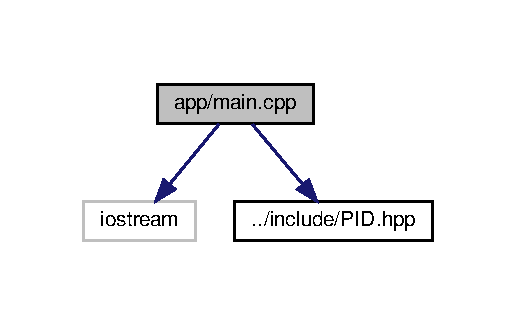
\includegraphics[width=248pt]{main_8cpp__incl}
\end{center}
\end{figure}
\subsection*{Functions}
\begin{DoxyCompactItemize}
\item 
\mbox{\Hypertarget{main_8cpp_ae66f6b31b5ad750f1fe042a706a4e3d4}\label{main_8cpp_ae66f6b31b5ad750f1fe042a706a4e3d4}} 
int {\bfseries main} ()
\end{DoxyCompactItemize}


\subsection{Detailed Description}
The program implements a \hyperlink{classPID}{P\+ID} controller for the input parameters. 

\begin{DoxyAuthor}{Author}
Pooja Kabra (\href{mailto:pkabra@terpmail.umd.edu}{\tt pkabra@terpmail.\+umd.\+edu}) 

Aditya Jadhav (\href{mailto:adi30jadhav@gmail.com}{\tt adi30jadhav@gmail.\+com}) 
\end{DoxyAuthor}
\begin{DoxyVersion}{Version}
2.\+0 
\end{DoxyVersion}
\begin{DoxyDate}{Date}
2021-\/10-\/02 
\end{DoxyDate}
\begin{DoxyCopyright}{Copyright}
Copyright (c) 2021 
\end{DoxyCopyright}

\hypertarget{PID_8cpp}{}\section{app/\+P\+ID.cpp File Reference}
\label{PID_8cpp}\index{app/\+P\+I\+D.\+cpp@{app/\+P\+I\+D.\+cpp}}


\hyperlink{classPID}{P\+ID} Class Implementation.  


{\ttfamily \#include \char`\"{}../include/\+P\+I\+D.\+hpp\char`\"{}}\newline
Include dependency graph for P\+I\+D.\+cpp\+:
\nopagebreak
\begin{figure}[H]
\begin{center}
\leavevmode
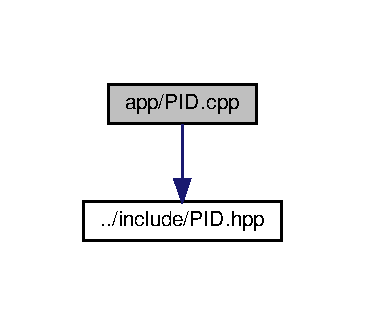
\includegraphics[width=175pt]{PID_8cpp__incl}
\end{center}
\end{figure}


\subsection{Detailed Description}
\hyperlink{classPID}{P\+ID} Class Implementation. 

\begin{DoxyAuthor}{Author}
Pooja Kabra (\href{mailto:pkabra@terpmail.umd.edu}{\tt pkabra@terpmail.\+umd.\+edu}) 

Aditya Jadhav (\href{mailto:adi30jadhav@gmail.com}{\tt adi30jadhav@gmail.\+com}) 
\end{DoxyAuthor}
\begin{DoxyVersion}{Version}
2.\+0 
\end{DoxyVersion}
\begin{DoxyDate}{Date}
2021-\/10-\/02 
\end{DoxyDate}
\begin{DoxyCopyright}{Copyright}
Copyright (c) 2021 
\end{DoxyCopyright}

\hypertarget{PID_8hpp}{}\section{include/\+P\+ID.hpp File Reference}
\label{PID_8hpp}\index{include/\+P\+I\+D.\+hpp@{include/\+P\+I\+D.\+hpp}}


\hyperlink{classPID}{P\+ID} Class header file.  


This graph shows which files directly or indirectly include this file\+:
\nopagebreak
\begin{figure}[H]
\begin{center}
\leavevmode
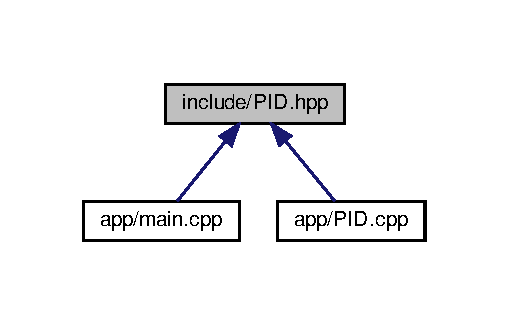
\includegraphics[width=244pt]{PID_8hpp__dep__incl}
\end{center}
\end{figure}
\subsection*{Classes}
\begin{DoxyCompactItemize}
\item 
class \hyperlink{classPID}{P\+ID}
\begin{DoxyCompactList}\small\item\em \hyperlink{classPID}{P\+ID} class with private gain variables and public compute method. \end{DoxyCompactList}\end{DoxyCompactItemize}


\subsection{Detailed Description}
\hyperlink{classPID}{P\+ID} Class header file. 

\begin{DoxyAuthor}{Author}
Pooja Kabra (\href{mailto:pkabra@terpmail.umd.edu}{\tt pkabra@terpmail.\+umd.\+edu}) 

Aditya Jadhav (\href{mailto:adi30jadhav@gmail.com}{\tt adi30jadhav@gmail.\+com}) 
\end{DoxyAuthor}
\begin{DoxyVersion}{Version}
2.\+0 
\end{DoxyVersion}
\begin{DoxyDate}{Date}
2021-\/10-\/02 
\end{DoxyDate}
\begin{DoxyCopyright}{Copyright}
Copyright (c) 2021 
\end{DoxyCopyright}

%--- End generated contents ---

% Index
\backmatter
\newpage
\phantomsection
\clearemptydoublepage
\addcontentsline{toc}{chapter}{Index}
\printindex

\end{document}
